\documentclass[tikz]{standalone}
\usepackage{booktabs}
\usepackage{times}
\usepackage{sourcecodepro}

\usetikzlibrary{positioning}
\tikzset{
  every node/.append style={font=\footnotesize},
}

\begin{document}
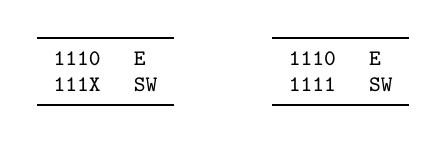
\begin{tikzpicture}
  % Non-orthogonal table
  \node (original) {
    \begin{tabular}{c l}
      \toprule
      \texttt{1110} & \texttt{E}\\
      \texttt{111X} & \texttt{SW}\\
      \bottomrule
    \end{tabular}
  };

  % Orthogonal equivalent
  \node (invalid) [right=of original] {
    \begin{tabular}{c l}
      \toprule
      \texttt{1110} & \texttt{E}\\
      \texttt{1111} & \texttt{SW}\\
      \bottomrule
    \end{tabular}
  };
\end{tikzpicture}
\end{document}
